%oppgavetekst

I oppgaven blir det gitt et ligningssystem: 
\begin{align}
{(x - {A_1})^2} + {(y - {B_1})^2} + {(z - {C_1})^2} &= {[c({t_1} - d)]^2} \nonumber \\ 
{(x - {A_2})^2} + {(y - {B_2})^2} + {(z - {C_2})^2} &= {[c({t_2} - d)]^2}  \nonumber \\
{(x - {A_3})^2} + {(y - {B_3})^2} + {(z - {C_3})^2} &= {[c({t_3} - d)]^2}  \nonumber \\
{(x - {A_4})^2} + {(y - {B_4})^2} + {(z - {C_4})^2} &= {[c({t_4} - d)]^2} \label{Ex1:system}
\end{align}

Det er ønskelig løse dette ligningssystemet slik at alle x, y, og z er uttrykt med d, slik at det kan lages kvadratiske ligninger i form av d, for så å løse dem med hensyn til d. I oppgaveteksten ble det fortalt at om man subtraherer de tre siste ligningene fra den første i (\ref{Ex1:system}), vil man få tre linneære ligninger. Vi starter med å subtrahere den andre ligningen med den første. 

\begin{multline}
{(x - {A_1})^2} - {(x - {A_2})^2} + {(y - {B_1})^2} - {(y - {B_2})^2} + {(z - {C_1})^2} - {(z - {C_2})^2} = 
{[c({t_1} - d)]^2} - {[c({t_2} - d)]^2}  \label{Ex1:linearEqs}
\end{multline}

Vi løser opp andregradsuttrykkene i (\ref{Ex1:linearEqs}) og setter uttrykket lik 0.
\begin{multline}
\\
({x^2} - 2{A_1}x + A_1^2) - ({x^2} - 2{A_2}x + A_2^2)  \\
+ \\
({y^2} - 2{B_1}y + B_1^2) - ({y^2} - 2{B_2}y + B_2^2) \\
+ \\
({z^2} - 2{C_1}z + C_1^2) - ({z^2} - 2{C_2}z + C_2^2)\\
- \\
({c^2}{t_1} - 2{t_1}{c^2} + {c^2}{d^2}) + ({c^2}{t_2} - 2{t_2}{c^2} + {c^2}{d^2}) \\
= \\
0 \\ \nonumber
\end{multline} 

Vi samler så utrykkene slik at x, y og z er samlet, mens de resterende konstantene blir samlet i en variabel kalt \\ $W = {A_1}^2 - {A_2}^2 + {B_1}^2 - {B_2}^2 + {C_1}^2 - {C_2}^2 + ({c^2}( - {t_1}^2 + {t_2}^2))$:  
\begin{multline}
- 2x({A_1} - {A_2}) - 2y({B_1} - {B_2}) - 2z({C_1} - {C_2}) + 2d{c^2}({t_1} - {t_2}) + W = 0
\end{multline}

Merk at ligning nr. 3 og 4 også skulle trekkes fra den første fra ligninssettet gitt i (\ref{Ex1:system}). De to nye ligningene vil gi de samme resultatene. De eneste forskjellene vil være koordinatene til satelittene. De tre ligningene blir:
\begin{align}
- 2x({A_1} - {A_2}) - 2y({B_1} - {B_2}) - 2z({C_1} - {C_2}) + 2d{c^2}({t_1} - {t_2}) + W &= 0 \nonumber \\
- 2x({A_1} - {A_3}) - 2y({B_1} - {B_3}) - 2z({C_1} - {C_3}) + 2d{c^2}({t_1} - {t_3}) + W &= 0  \nonumber\\
- 2x({A_1} - {A_4}) - 2y({B_1} - {B_4}) - 2z({C_1} - {C_4}) + 2d{c^2}({t_1} - {t_4}) + W &= 0 \nonumber \\ \label{Ex1:3equations}
\end{align}

Likningene blir så samlet slik at x-, y-, z-, og d-punktene blir samlet i hver sin vektor. Vektorene uttrykkes ved ${\vec u_x}, {\vec u_y}, {\vec u_z}$ og  ${\vec u_d}$, samt $\vec{w}$. 
\begin{align}
	{\vec u_x} &=  - 2\cdot[{A_1} - {A_2}, \enspace {A_1} - {A_3},  \enspace{A_1} - {A_4}]^T \nonumber \\
	{\vec u_y} &=  - 2\cdot[{B_1} - {B_2},  \enspace{B_1} - {B_3},  \enspace{B_1} - {B_4}]^T \nonumber \\
	{\vec u_z} &=  - 2\cdot[{C_1} - {C_2},  \enspace{C_1} - {C_3},  \enspace{C_1} - {C_4}]^T \nonumber \\
	{\vec u_d} &=  2c^2\cdot[{t_1} - {t_2},  \enspace{t_1} - {t_3},  \enspace{t_1} - {t_4}]^T \nonumber \\
	{\vec w}  &= 
	\begin{bmatrix}
		&{A_1}^2 - {A_2}^2 + {B_1}^2 - {B_2}^2 + {C_1}^2 - {C_2}^2 + ({c^2}( - {t_1}^2 + {t_2}^2)) \\
		&{A_1}^2 - {A_3}^2 + {B_1}^2 - {B_3}^2 + {C_1}^2 - {C_3}^2 + ({c^2}( - {t_1}^2 + {t_3}^2)) \\ 
		&{A_1}^2 - {A_4}^2 + {B_1}^2 - {B_4}^2 + {C_1}^2 - {C_4}^2 + ({c^2}( - {t_1}^2 + {t_4}^2))
	\end{bmatrix}\nonumber \\ \nonumber
\end{align}

Dette er skrevet i MatLab koden på følgende måte: 

\begin{lstlisting}
% Definerer Ux, Uy og Uz som regnet ut i teorien 
Ux = -2 *[A1 - A2; A1 - A3; A1 - A4];
Uy = -2 *[B1 - B2; B1 - B3; B1 - B4];
Uz = -2 *[C1 - C2; C1 - C3; C1 - C4];
Ud = 2 *(c^2)*[t1 - t2; t1 - t3; t1 - t4];
W = [A1^2 - A2^2 + B1^2 - B2^2 + C1^2 - C2^2 - (c^2)*(t1^2) + (c^2)*(t2^2); 
     A1^2 - A3^2 + B1^2 - B3^2 + C1^2 - C3^2 - (c^2)*(t1^2) + (c^2)*(t3^2); 
     A1^2 - A4^2 + B1^2 - B4^2 + C1^2 - C4^2 - (c^2)*(t1^2) + (c^2)*(t4^2)]; 
\end{lstlisting}

Vi får da uttrykket $x\cdot{\vec u_x} + y\cdot{\vec u_y} + z\cdot{\vec u_z} + d\cdot{\vec u_d} + {\vec w} = 0$. \newpage

%jorgen kommer her 

I boken står det at vi kan komme frem til en formel for x, uttrykt ved d, fra uttrykket $0=\text{det}[\vec{u}_y | \vec{u}_z | x\vec{u}_x + y\vec{u}_y + z\vec{u}_z + d\vec{u}_d + \vec{w}]$. Vi setter opp vektoren: 

\begin{align} \label{eq:detx}
	\text{det}[\vec{u}_y|\vec{u}_z |x\vec{u}_x + y\vec{u}_y + z\vec{u}_z + d\vec{u}_d + \vec{w}]=0
\end{align}

Vi ønsker å utlede et uttrykk for x fra denne determinanten. Determinanten for matrisen i likning \ref{eq:detx} kan skrives om på følgende måte: 

\begin{align}
	&\text{det}[\vec{u}_y|\vec{u}_z | x\vec{u}_x] \nonumber
	\\+ &\text{det}[\vec{u}_y|\vec{u}_z | y\vec{u}_y] \nonumber
	\\+ &\text{det}[\vec{u}_y|\vec{u}_z | z\vec{u}_z] \nonumber
	 \\+&\text{det}[\vec{u}_y|\vec{u}_z | d\vec{u}_d] \nonumber
	\\+ &\text{det}[\vec{u}_y|\vec{u}_z | \vec{w}]\nonumber
	\\&=0
\end{align}
%double end

Videre bruker vi loven som sier at matriser med repeterende kolonner er 0\cite{Determinants}. Da står vi igjen med: 

\begin{align} \label{eq:det_final}
	\text{det}[\vec{u}_y|\vec{u}_z | x\vec{u}_x] 
	+ \text{det}[\vec{u}_y|\vec{u}_z | d\vec{u}_d] 
	+ \text{det}[\vec{u}_y|\vec{u}_z | \vec{w}]
	=0
\end{align}

Den første delen av determinanten uttrykt i ligning \ref{eq:det_final} kan løses opp og få x på utsiden \cite{TheDeterminant}. Det samme kan gjøres hvor d inngår i matrisen. Da står vi igjen med: 

\begin{align}
	x\cdot\text{det}[\vec{u}_y|\vec{u}_z | \vec{u}_x] 
	+ d\cdot\text{det}[\vec{u}_y|\vec{u}_z | \vec{u}_d] 
	+ \text{det}[\vec{u}_y|\vec{u}_z | \vec{w}]
	=0 \nonumber 
	\\ 
	x\cdot\text{det}[\vec{u}_y|\vec{u}_z | \vec{u}_x] 
	= -d\cdot\text{det}[\vec{u}_y|\vec{u}_z | \vec{u}_d] 
	-\text{det}[\vec{u}_y|\vec{u}_z | \vec{w}]\nonumber 
\end{align}
Til slutt setter vi x alene. Da står vi igjen med: 

\begin{align}
    x=\frac{-d\cdot\text{det}[\vec{u}_y|\vec{u}_z | \vec{u}_d] 
	-\text{det}[\vec{u}_y|\vec{u}_z | \vec{w}]}{\text{det}[\vec{u}_y|\vec{u}_z | \vec{u}_x]}
\end{align}

For å finne uttrykk for henholdsvis y og z bruker vi samme metode, men med forskjellige utgangsvektorer. På grunn av at en matrise som inneholder lineært avhengige vektorer har determinant = 0 \cite{Determinants}, kan vi sette opp likninger for dette. Ved å veksle mellom å sette inn $\vec{u}_x$, $\vec{u}_y$ og $\vec{u}_z$ som de to første vektorene får vi gunstige startmatriser vi kan bruke for å uttrykke x, y og z med d. For y har vi følgende vektor som start: 

\begin{align} \label{eq:dety}
	\text{det}[\vec{u}_x|\vec{u}_z |x\vec{u}_x + y\vec{u}_y + z\vec{u}_z + d\vec{u}_d + \vec{w}]=0
\end{align}

For z har vi følgende vektor som start: 
\begin{align} \label{eq:detz}
	\text{det}[\vec{u}_x|\vec{u}_y |x\vec{u}_x + y\vec{u}_y + z\vec{u}_z + d\vec{u}_d + \vec{w}]=0
\end{align}

Bruker vi samme fremgangsmåte som for x, ender vi opp med følgende uttrykk for x, y og z: 

\begin{align}\label{eq:x}
    x=\frac{-d\cdot\text{det}[\vec{u}_y|\vec{u}_z | \vec{u}_d] 
	-\text{det}[\vec{u}_y|\vec{u}_z | \vec{w}]}{\text{det}[\vec{u}_y|\vec{u}_z | \vec{u}_x]}
\end{align}

\begin{align}\label{eq:y}
    y=\frac{-d\cdot\text{det}[\vec{u}_x|\vec{u}_z | \vec{u}_d] 
	-\text{det}[\vec{u}_x|\vec{u}_z | \vec{w}]}{\text{det}[\vec{u}_x|\vec{u}_z | \vec{u}_y]}
\end{align}

\begin{align}\label{eq:z}
    z=\frac{-d\cdot\text{det}[\vec{u}_x|\vec{u}_y | \vec{u}_d] 
	-\text{det}[\vec{u}_x|\vec{u}_y | \vec{w}]}{\text{det}[\vec{u}_x|\vec{u}_y | \vec{u}_z]}
\end{align}

Nå har vi altså fått uttrykt både x, y og z ved d. Vi kunne her ha uttrykt uttrykkene med den samme nevneren, ved å bruke loven som sier at vi kan endre fortegn til en determinant så lenge vi bytter plass på 2 rader \cite{TheDeterminant}. For nå å gå videre, setter vi disse inn i bokas likning 4.38. Dette vil resultere i en likning som inneholder d i første og andre grad, og vi kan derav finne d ved å bruke andregradsformelen. Med andre ord vil vi få ett utrykk som vi kan skrive som $Ad^2+Bd+C=0$ Andregradsformelen er gitt ved $d=\frac{-B \pm \sqrt{B^2-4AC}}{2A}$. Før vi setter uttrykkene vi har funnet for x, y og z inn i bokas likning 4.38, deler vi de opp i flere variabler for å gjøre uttrykket ryddigere. Vi setter

\begin{align}
	x_1&=\frac{-d\cdot\text{det}[\vec{u}_y|\vec{u}_z | \vec{u}_d]}{\text{det}[\vec{u}_y|\vec{u}_z | \vec{u}_x]}\nonumber 
\end{align}

\begin{align}
	x_2&=\frac{-d\cdot\text{det}[\vec{u}_y|\vec{u}_z | \vec{w}]}{\text{det}[\vec{u}_y|\vec{u}_z | \vec{u}_x]}\nonumber 
\end{align}

\begin{align}
	y_1&=\frac{-d\cdot\text{det}[\vec{u}_x|\vec{u}_z | \vec{u}_d]}{\text{det}[\vec{u}_x|\vec{u}_z | \vec{u}_y]}\nonumber 
\end{align}

\begin{align}
    y_2&=\frac{-d\cdot\text{det}[\vec{u}_x|\vec{u}_z | \vec{w}]}{\text{det}[\vec{u}_x|\vec{u}_z | \vec{u}_y]}\nonumber 
\end{align}

\begin{align}
    z_1&=\frac{-d\cdot\text{det}[\vec{u}_x|\vec{u}_y | \vec{u}_d]}{\text{det}[\vec{u}_x|\vec{u}_y | \vec{u}_z]}\nonumber
\end{align}

\begin{align}
    z_2&=\frac{-d\cdot\text{det}[\vec{u}_x|\vec{u}_y | \vec{w}]}{\text{det}[\vec{u}_x|\vec{u}_y | \vec{u}_z]}\nonumber 
\end{align}

I MatLab er dette kodet på følgende måte: 
\begin{lstlisting}
	%Dette bruker vi til å løse andregradslikningen for D. Definerer deler 
	%av uttrykket som forklart i teoridelen 
	x1 = -det([Uy Uz Ud])/det([Uy Uz Ux]);
	x2 = -det([Uy Uz W])/det([Uy Uz Ux]);

	y1 = -det([Ux Uz Ud])/det([Ux Uz Uy]);
	y2 = -det([Ux Uz W])/det([Ux Uz Uy]);

	z1 = -det([Ux Uy Ud])/det([Ux Uy Uz]);
	z2 = -det([Ux Uy W])/det([Ux Uy Uz]);
\end{lstlisting} 

Av dette følger det at $x=x_1+x_2$, $y=y_1+y_2$ og $z=z_1+z_2$. Setter vi nå dette inn i første likningen i bokas likning 4.38 får vi: 
\begin{multline}
	\\
    ((x_1+x_2)-A_1)^2+((y_1+y_2)-B_1)^2+((z_1+z_2)-C_1)^2\\
    =\\
    (c(t_1-d))^2 \\\nonumber
\end{multline}
\begin{multline}
	\\
  (x_1+x_2)^2-2A(x_1+x_2)+A^2+(y_1+y_2)^2-2B(y_1+y_2)+B^2\\
    +\\
    (z_1+z_2)^2-2C(z_1+z_2)+C^2-(c(t_1-d))^2\\
    =0 \nonumber 	\\
\end{multline}
\begin{multline}\label{eq:d_expanded}
    \\
    x_1^2+2x_1x_2+x_2^2-2Ax_1-2Ax_2+A^2+y_1^2+2y_1y_2+y_2^2-2By_1-2By_2+B^2\\
    +\\
    z_1^2+2z_1z_2+z_2^2-2Cz_1-2Cz_2+C^2-c^2t^2-c^22td-c^2d^2 \\
    = 0\\
\end{multline}
Som vi ser i utregning \ref{eq:d_expanded} har vi satt inn uttrykkene vi har funnet for x, y og z. Videre ønsker vi å samle alle leddene som vil få $d^2$ for seg, leddene med $d^1$ for seg og resten i en siste gruppe. Da vi ga verdier til $x_1$, $y_1$ og $z_1$, ser vi at det er bare disse leddene som inneholder en d. Det vil si at de eneste leddene hvor d blir i andre grad, er leddene hvor $x_1$, $y_1$ og $z_1$ er opphøyd i andre. Disse samler vi og setter inn i A i andregradsformelen. Videre vil alle leddene som inneholder d i første grad være der hvor $x_1$, $y_1$ og $z_1$ står i første grad. Disse samler vi i B i andregradsformelen. Vi har altså samlet alle koeffisientene som står foran $d^2$ i A, koeffisientene foran $d^1$ i B mens resten av leddene samles i C. A, B og C blir da som følger: 

\begin{align}
    A&=x_1^2+y_1^2+z_1^2-c^2 \\
    B&=2x_1x_2-2Ax_1+2y_1y_2-2By_1+2z_1z_2-2Cz_1-c^22t\\
    C&=x_2^2-2Ax_2+A^2+y_2^2-2By_2+B^2+z_2^2-2Cz_2+C^2-c^2t^2
\end{align}
Dette setter vi inn i andregradsformelen, og får derav 2 verdier for d. 

<<<<<<< Updated upstream
\begin{lstlisting}
A = (x1^2 + y1^2 + z1^2 - c^2);
B = 2*((x1*x2 - x1*A1) + (y1*y2 - y1*B2) + (z1*z2 - z1*C1)+ t1*c^2);
C = (x2^2 - 2*A1*x2 + A1^2) + (y2^2 -2*B1*y2 + B1^2) + (z2^2 - 2*C1*z2 + C1^2) - (c^2*t1^2);
dd(1) = (-B + sqrt(B^2 - 4*A*C))/(2*A);
dd(2) = (-B - sqrt(B^2 - 4*A*C))/(2*A);
\end{lstlisting}
Til slutt regner vi ut 2 verdier for x, y og z ved å bruke formlene \ref{eq:x}, \ref{eq:y} og \ref{eq:z}. Måten vi skiller mellom disse på er at vi sjekker om koordinatparene befinner seg omtrent på jordas overflate. Det vil alltid være ett sett av koordinater som ikke gjør det, og vi kan deretter utelukke dette settet. 
I MatLab er dette gjort på følgende måte: 

\begin{lstlisting}
	%Første løsning for x, y og z. Setter inn den ene verdien 
	%funnet d i uttrykket for x, y og z gitt i teorien:
	x = x1*dd(1) + x2;
	y = y1*dd(1) + y2;
	z = z1*dd(1) + z2;

	%Finner de andre verdiene
	xx = x1*dd(2) + x2;
	yy = y1*dd(2) + y2;
	zz = z1*dd(2) + z2;

	svar = [x y z;xx yy zz]; 

	%Finner hvilket sett som befinner seg på jordas overflate
	riktig_pos = 2;
	if (abs(svar(1,3) - 6371) < abs(svar(2,3) - 6371)) riktig_pos = 1; end

	%Setter riktige koordinater
	x= svar(riktig_pos,1); 
	y= svar(riktig_pos,2); 
	z= svar(riktig_pos,3); 
	d=dd(riktig_pos); 
	end
\end{lstlisting}

Resultatet av dette er vist i figur \ref{fig:task2result}. 

\begin{figure}[h]
    \centering
    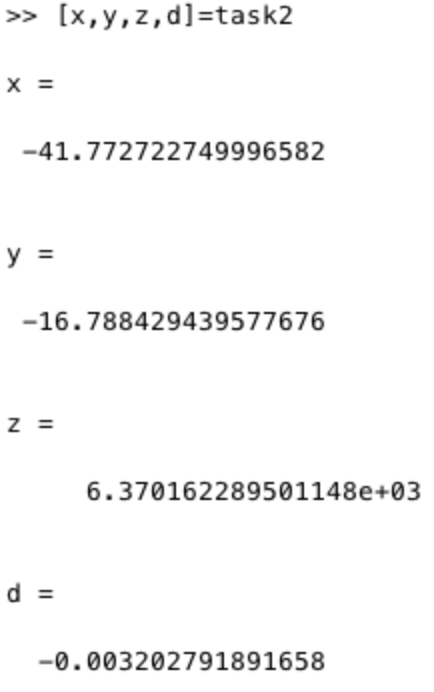
\includegraphics[width=0.4\textwidth]{sections/Exercise1/task2result.png}
    % 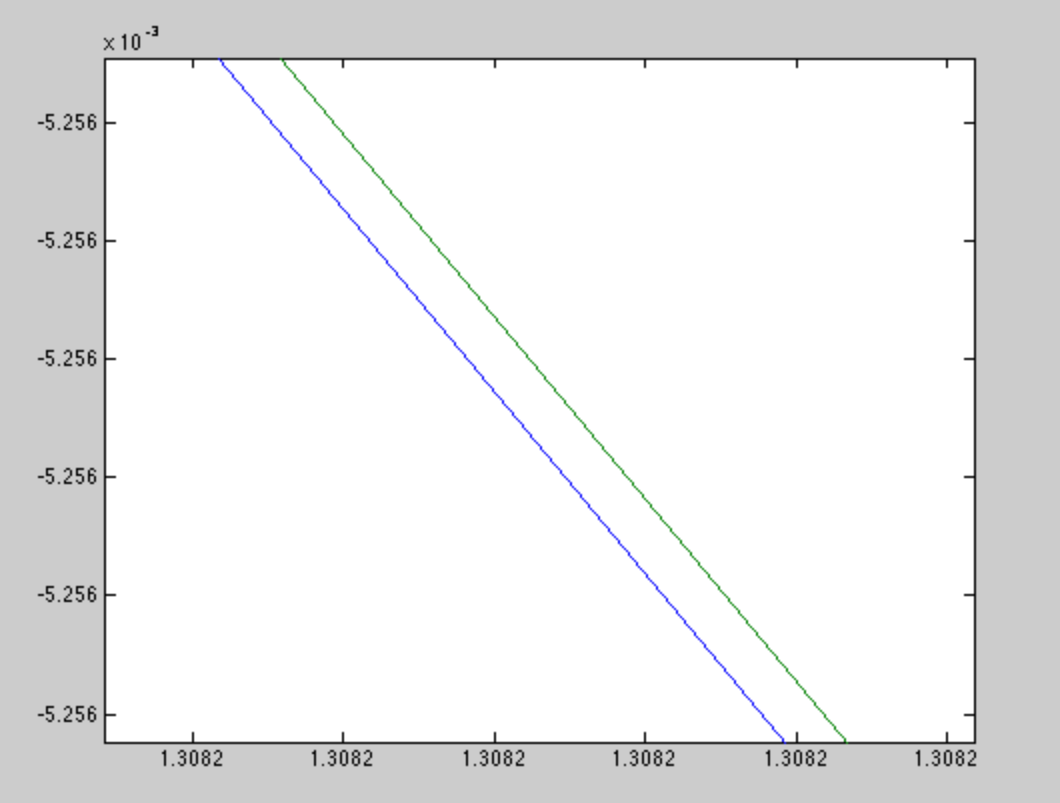
\includegraphics[width=0.4\textwidth]{errorplot2}
    \caption{Task2.m - result}
    \label{fig:task2result}
\end{figure}
=======
\begin{align}
    d=\frac{-(2x_1x_2-2Ax_1+2y_1y_2-2By_1+2z_1z_2-2Cz_1-c^22t) \pm \sqrt{(2x_1x_2-2Ax_1+2y_1y_2-2By_1+2z_1z_2-2Cz_1-c^22t)^2-4(x_1^2+y_1^2+z_1^2-c^2 )\cdot(x_2^2-2Ax_2+A^2+y_2^2-2By_2+B^2+z_2^2-2Cz_2+C^2-c^2t^2)}}{2A}
\end{align}
>>>>>>> Stashed changes
